\documentclass
[
a4paper,                      % Format A4
twoside,					  % double sided, alternative: oneside
12pt,                         % font size
abstract,		      % include if you want to use the abstract environment (if there is an abstract)
fleqn,                        % equations are aligned on the left side, comment if you want centered equations
%BCOR=5mm,                     % indention on left side because of the binding
%cleardoubleplain              % page numbers are printed on empty pages, comment if this is not desired
]
{scrartcl} % KOMA script package for scientific articles
%-----------------------------------------------------------------------------------
% Packages (do not touch if you don't know what you are doing)
%-----------------------------------------------------------------------------------
% symbols and orthography
\usepackage[latin1]{inputenc} % symbol set 
\usepackage[english,french]{babel}   	% englisch orthography
%\usepackage[french]{babel}	   % french					
%\usepackage[ngerman]{babel}   % german
\usepackage[T1]{fontenc}      % enables "Umlaute" (not really needed for English)
\usepackage[scaled=.90]{helvet}
%----------------------
% Creative Commons License
\usepackage[scale=2]{ccicons}
%----------------------
% graphics
\usepackage{graphicx}         	% package to include graphics (pdf, png, jpg)
\usepackage{subfig}			% package for subfigures
\usepackage{float}            		% Option [H] for fixing floats where you want them to be (not recommended unless you really need it)
\usepackage{tikz}
\usetikzlibrary{matrix,decorations.pathreplacing, calc, positioning,fit}
\usepackage{pgfplots} 
\usepackage{xcolor}  
%------------------------------
% math packages
\usepackage[cmex10]{amsmath}  
\usepackage{amstext}          
\usepackage{amsfonts}        
\usepackage{amssymb}          
\usepackage{bm}               
%-----------------------------
\usepackage{hyperref}
%--------------------------------
% other packages
\usepackage{enumerate}        % better listings
\usepackage{booktabs}         % nicer tables (see manual for usage)
\usepackage{textcomp}         % for \textdegree , \textcelsius , sometimes causes problems
%\usepackage{algorithm}        % for including algorithms
%\usepackage{algorithmic}      % same as above, but other package (check the manual for usage) 
%\usepackage{theorem}          % for theorems
\usepackage{pdfpages}         % include whole pages from pdf files
\usepackage{parskip}          % insert an empty line between paragraphs instead of an indented beginning
\usepackage[right]{eurosym}   % Euro symbol
%\usepackage[hyphens]{url}     %enables line breaks for URLs \url{http://www}
% set border size of page (comment if you want Latex to do this)
\usepackage[inner=3cm,%
								outer=2cm,%
								top=2.7cm,%
								bottom=3.2cm]{geometry}
\usepackage{setspace}		  % for a different line spacing
\usepackage{multirow}
\usepackage{rotating}
\usepackage{xcolor,colortbl}

\definecolor{Gray}{gray}{0.85}
\definecolor{LightCyan}{rgb}{0.88,1,1}
%-----------------------------------------------------------------------------------
% other stuff (do not touch, it is good that way !)
%-----------------------------------------------------------------------------------
\sloppy                   % avoids lines that are too long on the right side
% avoid "orphans"
\clubpenalty = 10000
% avoid "widows"
\widowpenalty = 10000
% this makes the table of content etc. look better
\renewcommand{\dotfill}{\leaders\hbox to 5pt{\hss.\hss}\hfill}

% avoid indentation of line after a paragraph
\setlength{\parindent}{0pt}
%-----------------------------------------------------------------------------------
%-----------------------------------------------------------------------------------

%Header and footer settings
% 
\usepackage{scrpage2} % see manual for usage
\pagestyle{scrheadings}
\automark[section]{section}
\ofoot{\pagemark} % ofoo
\ifoot{Research Plan} % ofoo
%\cfoot[]{\pagemark}
%\ihead{}
%\ohead{}
%\ohead{\headmark}
%\setheadtopline{2pt}
%\setheadsepline{0.5pt}
%\setfootsepline{0.5pt}

%%%%%%%%%%%%%%%%%%%%%%%%%%%%%%%%%%%%%%%%%%%%%%%%%%%%%%%%%%%%%%%%%%%%%%%%%%%%%%%
%%%%%%%%%%%%%%%%%%%%%%%%%%%%%%%%%%%%%%%%%%%%%%%%%%%%%%%%%%%%%%%%%%%%%%%%%%%%%%
%
% References with BibTeX
%
\usepackage{natbib}
\bibliographystyle{apalike}
%\bibliographystyle{elsart-harv}
\setlength{\bibsep}{3mm}                  % spacing of the entries in the references
%
% look at the chapterbib package if you want to use a separate bibliography for each chapter
%
%%%%%%%%%%%%%%%%%%%%%%%%%%%%%%%%%%%%%%%%%%%%%%%%%%%%%%%%%%%%%%%%%%%%%%%%%%%%%%
%%%%%%%%%%%%%%%%%%%%%%%%%%%%%%%%%%%%%%%%%%%%%%%%%%%%%%%%%%%%%%%%%%%%%%%%%%%%%%
%
% some other stuff...
%
\setlength{\unitlength}{1cm}
\setlength{\oddsidemargin}{0.3cm}
\setlength{\evensidemargin}{0.3cm}
\setlength{\textwidth}{15.5cm}
\setlength{\topmargin}{0cm}
\setlength{\textheight}{22cm}
\columnsep 0.5cm

%%%%%%%%%%%%%%%%%%%%%%%%%%%%%%%%%%%%%%%%%%%%%%%%

% just compile particular parts
%
%\includeonly{./SUMMARY/summary} % put in here the path of the file you want to include only
%%%%%%%%%%%%%%%%%%%%%%%%%%%%%%%%%%%%%%%%%%%%%%%%%%%%%%%%%%%%%%%%%%%%%%%%%%%%%%

% define own commands
\newcommand{\brac}[1]{\left(#1\right)}		

%-----------------------------------------------------------------------------------%
%-----------------------------------------------------------------------------------%
%-----------------------------------------------------------------------------------%
%                                    START OF THE DOCUMENT                                %
%-----------------------------------------------------------------------------------%
%-----------------------------------------------------------------------------------%
%-----------------------------------------------------------------------------------%

\begin{document}

%------------------------------------------------%
%------------------------------------------------%
%                  Front Matter                         %
%------------------------------------------------%
%------------------------------------------------%

%------------------------------------------------%
%                 Title Page                               
%------------------------------------------------%

\clearscrheadings
\pagestyle{scrheadings}
\manualmark
%\ofoot{\pagemark} % ofoo
%\ifoot{Research Plan} % ofoo
%\cfoot[]{\pagemark}
%\ihead{}
%\ohead{}
\ihead{
\includegraphics[height=1.25cm]{logo-eeigm-ht90.png}\hspace{2.75cm}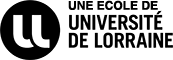
\includegraphics[height=1.25cm]{label-logo-ul.png}}
\ifoot{\noindent\makebox[\linewidth]{\rule{\textwidth}{0.4pt}}\\\textsc{EEIGM - 6, rue Bastien-Lepage BP 10630 - F-54010 Nancy Cedex}}

%\ohead{Abstract}
%\setheadtopline{2pt}
\setheadsepline{0.5pt}
%\setfootsepline{0.5pt}

\begin{center}

\vspace*{2cm}

\begin{Large}
\textbf{\textsc{EEIGM}}\\[0.75ex]
\end{Large}

\begin{large}
\textbf{\'Ecole Europ\'eenne d'Ing\'enieurs en G\'enie des Mat\'eriaux}\\[0.75ex]
\end{large}

\vspace{2cm}

\begin{large}
\textbf{$2^{`eme}$ Ann\'ee, $1^{er}$ Semestre}\\[0.75ex]
\end{large}
\vspace*{0.5cm}

\begin{Large}
\textbf{\textsc{M\'ecanique du Solide D\'eformable}}\\[0.75ex]
\end{Large}
\vspace*{0.5cm}

\begin{Large}
\textbf{\textsc{Notes du Cours}}\\[0.75ex]
\end{Large}
\vspace*{2.5cm}

\begin{large}
\textbf{Luca Di Stasio}\\[0.75ex]
\end{large}

\vspace{2cm}
%\begin{flushright}
%\begin{tabular}{l l }
%{\large \textbf{Author(s):}} & {\large Luca DI STASIO}\\
%\end{tabular}
%\end{flushright}

\begin{large}
\ccLogo\ccAttribution\ccNonCommercial\\[0.75ex]
Cette oeuvre est mise \`a disposition selon les termes de la\\ \href{https://creativecommons.org/licenses/by-nc/4.0/deed.fr}{Licence Creative Commons Attribution - Pas d'Utilisation Commerciale 4.0 International}.\\[0.75ex]
\end{large}

\vspace*{3cm}


{\large \textbf{\today}}\\
%\textsc{DEFENSE LOCATION}\\

%------------------------------------------------
% Committee members:
%\textbf{\textsc{Committee Members}}\\[0.75ex]
%\textsc{NAME AND AFFILIATION}\\
%\textsc{NAME AND AFFILIATION}\\
%\textsc{NAME AND AFFILIATION}\\
%\textsc{ }\\

\end{center}

\newpage

%------------------------------------------------%
%            Table of Contents
%------------------------------------------------%

\pagenumbering{roman}

\setcounter{page}{1}

\clearscrheadings
\pagestyle{scrheadings}
\manualmark
\ofoot{\\ \pagemark} % ofoo
\ifoot{} % ofoo
%\cfoot[]{\pagemark}
%\ihead{}
%\ohead{}
\ohead{Table des mati\`eres}
\setheadtopline{2pt}
\setheadsepline{0.5pt}
\setfootsepline{0.5pt}

\hypertarget{contents}{}
\tableofcontents 

\cleardoublepage

%------------------------------------------------%
%            List of Acronyms
%------------------------------------------------%

%\clearscrheadings
%\pagestyle{scrheadings}
%\manualmark
%\ofoot{\\ \pagemark} % ofoo
%\ifoot{} % ofoo
%%\cfoot[]{\pagemark}
%%\ihead{}
%%\ohead{}
%\ohead{List of Acronyms}
%\setheadtopline{2pt}
%\setheadsepline{0.5pt}
%\setfootsepline{0.5pt}
%
%\section*{List of Acronyms}
%\addcontentsline{toc}{section}{List of Acronyms}
%
%\cleardoublepageusingstyle{scrheadings}

%------------------------------------------------%
%            List of Symbols
%------------------------------------------------%

%\clearscrheadings
%\pagestyle{scrheadings}
%\manualmark
%\ofoot{\\ \pagemark} % ofoo
%\ifoot{} % ofoo
%%\cfoot[]{\pagemark}
%%\ihead{}
%%\ohead{}
%\ohead{List of Symbols}
%\setheadtopline{2pt}
%\setheadsepline{0.5pt}
%\setfootsepline{0.5pt}
%
%\section*{List of Symbols}
%\addcontentsline{toc}{section}{List of Symbols}
%
%\cleardoublepageusingstyle{scrheadings}

%------------------------------------------------%
%                       Abstract
%------------------------------------------------%

%\clearscrheadings
%\pagestyle{scrheadings}
%\manualmark
%\ofoot{\\ \pagemark} % ofoo
%\ifoot{} % ofoo
%%\cfoot[]{\pagemark}
%%\ihead{}
%%\ohead{}
%\ohead{Abstract}
%\setheadtopline{2pt}
%\setheadsepline{0.5pt}
%\setfootsepline{0.5pt}
%
%\section*{Abstract}
%\addcontentsline{toc}{section}{Abstract}
%
%\cleardoublepageusingstyle{scrheadings}

%------------------------------------------------%
%------------------------------------------------%
%                   Main Matter                          %
%------------------------------------------------%
%------------------------------------------------%

\pagenumbering{arabic}

\setcounter{page}{1}

%------------------------------------------------%
%                   Introduction
%------------------------------------------------%

\clearscrheadings
\pagestyle{scrheadings}
\manualmark
\ofoot{\\\pagemark} % ofoo
\ifoot{\hyperlink{contents}{Retourner \'a la table des mati\`eres}} % ofoo
%\cfoot[]{\pagemark}
\ihead{\hyperlink{contents}{Retourner \'a la table des mati\`eres}}
\ohead{Introduction}
\setheadtopline{2pt}
\setheadsepline{0.5pt}
\setfootsepline{0.5pt}

\section{Syst\`emes de coordonn\'ees curvilignes}

\subsection{Formulation analytique}

\begin{equation}
\begin{cases}
x=x\left(\xi,\eta,\zeta\right)\\
y=y\left(\xi,\eta,\zeta\right)\\
z=z\left(\xi,\eta,\zeta\right)
\end{cases}\longleftrightarrow\begin{cases}
\xi=\xi\left(x,y,z\right)\\
\eta=\eta\left(x,y,z\right)\\
\zeta=\zeta\left(x,y,z\right)
\end{cases}
\end{equation}

\subsection{Le d\'eplacement infinit\'esimal d'un point et le jacobien de la transformation}

\begin{equation}
\mathbf{r}=\begin{bmatrix}
x\\
y\\
z\\
\end{bmatrix}=\begin{bmatrix}
\xi\\
\eta\\
\zeta\\
\end{bmatrix}
\end{equation}

\begin{equation}
d\mathbf{r}=\begin{bmatrix}
dx\\
dy\\
dz\\
\end{bmatrix}
\end{equation}

\begin{equation}
\begin{cases}
dx=\frac{\partial x}{\partial\xi}d \xi+\frac{\partial x}{\partial\eta}d \eta+\frac{\partial x}{\partial\zeta}d \zeta\\
dy=\frac{\partial y}{\partial\xi}d \xi+\frac{\partial y}{\partial\eta}d \eta+\frac{\partial y}{\partial\zeta}d \zeta\\
dz=\frac{\partial z}{\partial\xi}d \xi+\frac{\partial z}{\partial\eta}d \eta+\frac{\partial z}{\partial\zeta}d \zeta\\
\end{cases}
\end{equation}

\begin{equation}
d\mathbf{r}=\begin{bmatrix}
dx\\
dy\\
dz\\
\end{bmatrix}=\underbrace{\begin{bmatrix}
\frac{\partial x}{\partial\xi}&\frac{\partial x}{\partial\eta}&\frac{\partial x}{\partial\zeta}\\
\frac{\partial y}{\partial\xi}&\frac{\partial y}{\partial\eta}&\frac{\partial y}{\partial\zeta}\\
\frac{\partial z}{\partial\xi}&\frac{\partial z}{\partial\eta}&\frac{\partial z}{\partial\zeta}\\
\end{bmatrix}}_{\mathbf{J}}\begin{bmatrix}
d\xi\\
d\eta\\
d\zeta\\
\end{bmatrix}=\mathbf{J}\begin{bmatrix}
d\xi\\
d\eta\\
d\zeta\\
\end{bmatrix}
\end{equation}

\subsection{Les vecteurs du rep\`ere local naturel (base covariante)}

\tikzset{node style ge/.style={circle}}

\begin{center}
\begin{tabular}{ccc}
\begin{tikzpicture}
\matrix (A) [matrix of math nodes,left delimiter={[},right delimiter={]}] 
{ \frac{\partial x}{\partial\xi}&\frac{\partial x}{\partial\eta}&\frac{\partial x}{\partial\zeta}\\
\frac{\partial y}{\partial\xi}&\frac{\partial y}{\partial\eta}&\frac{\partial y}{\partial\zeta}\\
\frac{\partial z}{\partial\xi}&\frac{\partial z}{\partial\eta}&\frac{\partial z}{\partial\zeta}\\
};
\draw [blue!50!black,fill=blue!10!white,fill opacity =0.25] (A-1-1.north east) to (A-3-1.south east) to (A-3-1.south west) to (A-1-1.north west) to (A-1-1.north east);
\end{tikzpicture}
&
\begin{tikzpicture}
\matrix (A) [matrix of math nodes,left delimiter={[},right delimiter={]}] 
{ \frac{\partial x}{\partial\xi}&\frac{\partial x}{\partial\eta}&\frac{\partial x}{\partial\zeta}\\
\frac{\partial y}{\partial\xi}&\frac{\partial y}{\partial\eta}&\frac{\partial y}{\partial\zeta}\\
\frac{\partial z}{\partial\xi}&\frac{\partial z}{\partial\eta}&\frac{\partial z}{\partial\zeta}\\
};
\draw [green!30!black,fill=green!10!white,fill opacity =0.25] (A-1-2.north east) to (A-3-2.south east) to (A-3-2.south west) to (A-1-2.north west) to (A-1-2.north east);
\end{tikzpicture}
&
\begin{tikzpicture}
\matrix (A) [matrix of math nodes,left delimiter={[},right delimiter={]}] 
{ \frac{\partial x}{\partial\xi}&\frac{\partial x}{\partial\eta}&\frac{\partial x}{\partial\zeta}\\
\frac{\partial y}{\partial\xi}&\frac{\partial y}{\partial\eta}&\frac{\partial y}{\partial\zeta}\\
\frac{\partial z}{\partial\xi}&\frac{\partial z}{\partial\eta}&\frac{\partial z}{\partial\zeta}\\
};
\draw [purple!50!black,fill=purple!10!white,fill opacity =0.25] (A-1-3.north east) to (A-3-3.south east) to (A-3-3.south west) to (A-1-3.north west) to (A-1-3.north east);
\end{tikzpicture}
\\
$\color{blue!50!black} \frac{\partial \mathbf{r}}{\partial\xi}$&$\color{green!30!black} \frac{\partial \mathbf{r}}{\partial\eta}$&$\color{purple!50!black} \frac{\partial \mathbf{r}}{\partial\zeta}$\\
\end{tabular}
\end{center}

\begin{equation}
\begin{aligned}
\mathbf{i}_{\xi}=&\frac{1}{\lvert\lvert\frac{\partial \mathbf{r}}{\partial\xi}\rvert\rvert}\frac{\partial \mathbf{r}}{\partial\xi}=\frac{1}{\sqrt{\left(\frac{\partial x}{\partial\xi}\right)^{2}+\left(\frac{\partial y}{\partial\xi}\right)^{2}+\left(\frac{\partial z}{\partial\xi}\right)^{2}}}\begin{bmatrix}
\frac{\partial x}{\partial\xi}\\[5pt]
\frac{\partial y}{\partial\xi}\\[5pt]
\frac{\partial z}{\partial\xi}\end{bmatrix}\\
\mathbf{j}_{\eta}=&\frac{1}{\lvert\lvert\frac{\partial \mathbf{r}}{\partial\eta}\rvert\rvert}\frac{\partial \mathbf{r}}{\partial\eta}=\frac{1}{\sqrt{\left(\frac{\partial x}{\partial\eta}\right)^{2}+\left(\frac{\partial y}{\partial\eta}\right)^{2}+\left(\frac{\partial z}{\partial\eta}\right)^{2}}}\begin{bmatrix}
\frac{\partial x}{\partial\eta}\\[5pt]
\frac{\partial y}{\partial\eta}\\[5pt]
\frac{\partial z}{\partial\eta}\end{bmatrix}\\
\mathbf{k}_{\zeta}=&\frac{1}{\lvert\lvert\frac{\partial \mathbf{r}}{\partial\zeta}\rvert\rvert}\frac{\partial \mathbf{r}}{\partial\zeta}=\frac{1}{\sqrt{\left(\frac{\partial x}{\partial\zeta}\right)^{2}+\left(\frac{\partial y}{\partial\zeta}\right)^{2}+\left(\frac{\partial z}{\partial\zeta}\right)^{2}}}\begin{bmatrix}
\frac{\partial x}{\partial\zeta}\\[5pt]
\frac{\partial y}{\partial\zeta}\\[5pt]
\frac{\partial z}{\partial\zeta}\end{bmatrix}
\end{aligned}
\end{equation}

\subsection{L'\'el\'ement infinit\'esimal de ligne et le tenseur m\'etrique}

\begin{equation}
dl^{2}=d\mathbf{r}^{T}d\mathbf{r}=\begin{bmatrix}
dx&
dy&
dz\\
\end{bmatrix}\begin{bmatrix}
dx\\
dy\\
dz\\
\end{bmatrix}=dx^{2}+dy^{2}+dz^{2}
\end{equation}

\begin{equation}
\footnotesize
\begin{aligned}
dl^{2}&=d\mathbf{r}^{T}d\mathbf{r}=\begin{bmatrix}
d\xi&
d\eta&
d\zeta\\
\end{bmatrix}\mathbf{J}^{T}\mathbf{J}\begin{bmatrix}
d\xi\\
d\eta\\
d\zeta\\
\end{bmatrix}=\\&=\begin{bmatrix}
d\xi&
d\eta&
d\zeta\\
\end{bmatrix}\begin{bmatrix}
\frac{\partial x}{\partial\xi}&\frac{\partial y}{\partial\xi}&\frac{\partial z}{\partial\xi}\\
\frac{\partial x}{\partial\eta}&\frac{\partial y}{\partial\eta}&\frac{\partial z}{\partial\eta}\\
\frac{\partial x}{\partial\zeta}&\frac{\partial y}{\partial\zeta}&\frac{\partial z}{\partial\zeta}\\
\end{bmatrix}\begin{bmatrix}
\frac{\partial x}{\partial\xi}&\frac{\partial x}{\partial\eta}&\frac{\partial x}{\partial\zeta}\\
\frac{\partial y}{\partial\xi}&\frac{\partial y}{\partial\eta}&\frac{\partial y}{\partial\zeta}\\
\frac{\partial z}{\partial\xi}&\frac{\partial z}{\partial\eta}&\frac{\partial z}{\partial\zeta}\\
\end{bmatrix}\begin{bmatrix}
d\xi\\
d\eta\\
d\zeta\\
\end{bmatrix}=\\&=\begin{bmatrix}
d\xi&
d\eta&
d\zeta\\
\end{bmatrix}\underbrace{\begin{bmatrix}
\left(\frac{\partial x}{\partial\xi}\right)^{2}+\left(\frac{\partial y}{\partial\xi}\right)^{2}+\left(\frac{\partial z}{\partial\xi}\right)^{2}&\frac{\partial x}{\partial\xi}\frac{\partial x}{\partial\eta}+\frac{\partial y}{\partial\xi}\frac{\partial y}{\partial\eta}+\frac{\partial z}{\partial\xi}\frac{\partial z}{\partial\eta}&\frac{\partial x}{\partial\xi}\frac{\partial x}{\partial\zeta}+\frac{\partial y}{\partial\xi}\frac{\partial y}{\partial\zeta}+\frac{\partial z}{\partial\xi}\frac{\partial z}{\partial\zeta}\\
\frac{\partial x}{\partial\xi}\frac{\partial x}{\partial\eta}+\frac{\partial y}{\partial\xi}\frac{\partial y}{\partial\eta}+\frac{\partial z}{\partial\xi}\frac{\partial z}{\partial\eta}&\left(\frac{\partial x}{\partial\eta}\right)^{2}+\left(\frac{\partial y}{\partial\eta}\right)^{2}+\left(\frac{\partial z}{\partial\eta}\right)^{2}&\frac{\partial x}{\partial\eta}\frac{\partial x}{\partial\zeta}+\frac{\partial y}{\partial\eta}\frac{\partial y}{\partial\zeta}+\frac{\partial z}{\partial\eta}\frac{\partial z}{\partial\zeta}\\
\frac{\partial x}{\partial\xi}\frac{\partial x}{\partial\zeta}+\frac{\partial y}{\partial\xi}\frac{\partial y}{\partial\zeta}+\frac{\partial z}{\partial\xi}\frac{\partial z}{\partial\zeta}&\frac{\partial x}{\partial\eta}\frac{\partial x}{\partial\zeta}+\frac{\partial y}{\partial\eta}\frac{\partial y}{\partial\zeta}+\frac{\partial z}{\partial\eta}\frac{\partial z}{\partial\zeta}&\left(\frac{\partial x}{\partial\zeta}\right)^{2}+\left(\frac{\partial y}{\partial\zeta}\right)^{2}+\left(\frac{\partial z}{\partial\zeta}\right)^{2}\\
\end{bmatrix}}_{\mathbf{g}}\begin{bmatrix}
d\xi\\
d\eta\\
d\zeta\\
\end{bmatrix}
\end{aligned}
\end{equation}

\subsection{L'\'el\'ement infinit\'esimal de volume}

\begin{equation}
dV=\frac{\partial \mathbf{r}}{\partial\xi}d\xi\cdot\left(\frac{\partial \mathbf{r}}{\partial\eta}d\eta\wedge\frac{\partial \mathbf{r}}{\partial\zeta}d\zeta\right)=det\begin{bmatrix}
\left(\frac{\partial \mathbf{r}}{\partial\xi}\right)^{T}\\
\left(\frac{\partial \mathbf{r}}{\partial\eta}\right)^{T}\\
\left(\frac{\partial \mathbf{r}}{\partial\zeta}\right)^{T}\\
\end{bmatrix}d\xi d\eta d\zeta=det\left(\mathbf{J}^{T}\right)d\xi d\eta d\zeta
\end{equation}

\subsection{Les vecteurs de la base contravariante et le gradient d'un fonction scalaire $\nabla f$}

\begin{equation}
f\left(x,y,z\right)=f\left(x\left(\xi,\eta,\zeta\right),y\left(\xi,\eta,\zeta\right),z\left(\xi,\eta,\zeta\right)\right)
\end{equation}

\begin{equation}
f\left(\xi,\eta,\zeta\right)=f\left(\xi\left(x,y,z\right),\eta\left(x,y,z\right),\zeta\left(x,y,z\right)\right)
\end{equation}

\begin{equation}
\nabla f_{xyz}=\begin{bmatrix}
\frac{\partial f}{\partial x}\\[5pt]
\frac{\partial f}{\partial y}\\[5pt]
\frac{\partial f}{\partial z}
\end{bmatrix}=\frac{\partial f}{\partial x}\begin{bmatrix}
1\\[5pt]
0\\[5pt]
0
\end{bmatrix}+\frac{\partial f}{\partial y}\begin{bmatrix}
0\\[5pt]
1\\[5pt]
0
\end{bmatrix}+\frac{\partial f}{\partial z}\begin{bmatrix}
0\\[5pt]
0\\[5pt]
1
\end{bmatrix}=\frac{\partial f}{\partial x}\mathbf{i}^{x}+\frac{\partial f}{\partial y}\mathbf{j}^{y}+\frac{\partial f}{\partial z}\mathbf{k}^{z}
\end{equation}

\begin{equation}
\nabla f=\begin{bmatrix}
\frac{\partial f}{\partial x}\\[5pt]
\frac{\partial f}{\partial y}\\[5pt]
\frac{\partial f}{\partial z}
\end{bmatrix}=\begin{bmatrix}
\frac{\partial f}{\partial\xi}\frac{\partial\xi}{\partial x}+\frac{\partial f}{\partial\eta}\frac{\partial\eta}{\partial x}+\frac{\partial f}{\partial\zeta}\frac{\partial\zeta}{\partial x}\\[5pt]
\frac{\partial f}{\partial\xi}\frac{\partial\xi}{\partial y}+\frac{\partial f}{\partial\eta}\frac{\partial\eta}{\partial y}+\frac{\partial f}{\partial\zeta}\frac{\partial\zeta}{\partial y}\\[5pt]
\frac{\partial f}{\partial\xi}\frac{\partial\xi}{\partial z}+\frac{\partial f}{\partial\eta}\frac{\partial\eta}{\partial z}+\frac{\partial f}{\partial\zeta}\frac{\partial\zeta}{\partial z}
\end{bmatrix}=\frac{\partial f}{\partial\xi}\begin{bmatrix}
\frac{\partial\xi}{\partial x}\\[5pt]
\frac{\partial\xi}{\partial y}\\[5pt]
\frac{\partial\xi}{\partial z}\end{bmatrix}+\frac{\partial f}{\partial\eta}\begin{bmatrix}
\frac{\partial\eta}{\partial x}\\[5pt]
\frac{\partial\eta}{\partial y}\\[5pt]
\frac{\partial\eta}{\partial z}\end{bmatrix}+\frac{\partial f}{\partial\zeta}\begin{bmatrix}
\frac{\partial\zeta}{\partial x}\\[5pt]
\frac{\partial\zeta}{\partial y}\\[5pt]
\frac{\partial\zeta}{\partial z}
\end{bmatrix}
\end{equation}

\begin{equation}
\begin{aligned}
\mathbf{i}^{\xi}=&\frac{1}{\sqrt{\left(\frac{\partial\xi}{\partial x}\right)^{2}+\left(\frac{\partial\xi}{\partial y}\right)^{2}+\left(\frac{\partial\xi}{\partial z}\right)^{2}}}\begin{bmatrix}
\frac{\partial\xi}{\partial x}\\[5pt]
\frac{\partial\xi}{\partial y}\\[5pt]
\frac{\partial\xi}{\partial z}\end{bmatrix}\\
\mathbf{j}^{\eta}=&\frac{1}{\sqrt{\left(\frac{\partial\eta}{\partial x}\right)^{2}+\left(\frac{\partial\eta}{\partial y}\right)^{2}+\left(\frac{\partial\eta}{\partial z}\right)^{2}}}\begin{bmatrix}
\frac{\partial\eta}{\partial x}\\[5pt]
\frac{\partial\eta}{\partial y}\\[5pt]
\frac{\partial\eta}{\partial z}\end{bmatrix}\\
\mathbf{k}^{\zeta}=&\frac{1}{\sqrt{\left(\frac{\partial\zeta}{\partial x}\right)^{2}+\left(\frac{\partial\zeta}{\partial y}\right)^{2}+\left(\frac{\partial\zeta}{\partial z}\right)^{2}}}\begin{bmatrix}
\frac{\partial\zeta}{\partial x}\\[5pt]
\frac{\partial\zeta}{\partial y}\\[5pt]
\frac{\partial\zeta}{\partial z}
\end{bmatrix}
\end{aligned}
\end{equation}

\begin{equation}
\begin{aligned}
\nabla_{\xi\eta\zeta} f=&\frac{\partial f}{\partial\xi}\sqrt{\left(\frac{\partial\xi}{\partial x}\right)^{2}+\left(\frac{\partial\xi}{\partial y}\right)^{2}+\left(\frac{\partial\xi}{\partial z}\right)^{2}}\cdot\mathbf{i}^{\xi}+\\
&+\frac{\partial f}{\partial\eta}\sqrt{\left(\frac{\partial\eta}{\partial x}\right)^{2}+\left(\frac{\partial\eta}{\partial y}\right)^{2}+\left(\frac{\partial\eta}{\partial z}\right)^{2}}\cdot\mathbf{j}^{\eta}+\\
&+\frac{\partial f}{\partial\zeta}\sqrt{\left(\frac{\partial\zeta}{\partial x}\right)^{2}+\left(\frac{\partial\zeta}{\partial y}\right)^{2}+\left(\frac{\partial\zeta}{\partial z}\right)^{2}}\cdot\mathbf{k}^{\zeta}=\\
=&\begin{bmatrix}
\frac{\partial f}{\partial\xi}\sqrt{\left(\frac{\partial\xi}{\partial x}\right)^{2}+\left(\frac{\partial\xi}{\partial y}\right)^{2}+\left(\frac{\partial\xi}{\partial z}\right)^{2}}\\[10pt]
\frac{\partial f}{\partial\eta}\sqrt{\left(\frac{\partial\eta}{\partial x}\right)^{2}+\left(\frac{\partial\eta}{\partial y}\right)^{2}+\left(\frac{\partial\eta}{\partial z}\right)^{2}}\\[10pt]
\frac{\partial f}{\partial\zeta}\sqrt{\left(\frac{\partial\zeta}{\partial x}\right)^{2}+\left(\frac{\partial\zeta}{\partial y}\right)^{2}+\left(\frac{\partial\zeta}{\partial z}\right)^{2}}
\end{bmatrix}
\end{aligned}
\end{equation}

\subsection{L'op\'erateur laplacien $\nabla^{2}$}

\begin{equation}
f\left(x,y,z\right)=f\left(x\left(\xi,\eta,\zeta\right),y\left(\xi,\eta,\zeta\right),z\left(\xi,\eta,\zeta\right)\right)
\end{equation}

\begin{equation}
f\left(\xi,\eta,\zeta\right)=f\left(\xi\left(x,y,z\right),\eta\left(x,y,z\right),\zeta\left(x,y,z\right)\right)
\end{equation}

\begin{equation}
\nabla_{xyz}^{2}f\left(x,y,z\right)=\frac{\partial^{2} f}{\partial x^{2}}+\frac{\partial^{2} f}{\partial y^{2}}+\frac{\partial^{2} f}{\partial z^{2}}
\end{equation}

\begin{equation}
\begin{cases}
\frac{\partial f}{\partial x}=\frac{\partial f}{\partial\xi}\frac{\partial\xi}{\partial x}+\frac{\partial f}{\partial\eta}\frac{\partial\eta}{\partial x}+\frac{\partial f}{\partial\zeta}\frac{\partial\zeta}{\partial x}\\[5pt]
\frac{\partial f}{\partial y}=\frac{\partial f}{\partial\xi}\frac{\partial\xi}{\partial y}+\frac{\partial f}{\partial\eta}\frac{\partial\eta}{\partial y}+\frac{\partial f}{\partial\zeta}\frac{\partial\zeta}{\partial y}\\[5pt]
\frac{\partial f}{\partial z}=\frac{\partial f}{\partial\xi}\frac{\partial\xi}{\partial z}+\frac{\partial f}{\partial\eta}\frac{\partial\eta}{\partial z}+\frac{\partial f}{\partial\zeta}\frac{\partial\zeta}{\partial z}
\end{cases}
\end{equation}

\begin{equation}
\begin{cases}
\frac{\partial^{2} f}{\partial x^{2}}&=\frac{\partial}{\partial x}\left(\frac{\partial f}{\partial\xi}\frac{\partial\xi}{\partial x}+\frac{\partial f}{\partial\eta}\frac{\partial\eta}{\partial x}+\frac{\partial f}{\partial\zeta}\frac{\partial\zeta}{\partial x}\right)=\\[5pt]
&=\frac{\partial}{\partial x}\left(\frac{\partial f}{\partial\xi}\right)\frac{\partial\xi}{\partial x}+\frac{\partial}{\partial x}\left(\frac{\partial f}{\partial\eta}\right)\frac{\partial\eta}{\partial x}+\frac{\partial}{\partial x}\left(\frac{\partial f}{\partial\zeta}\right)\frac{\partial\zeta}{\partial x}+\frac{\partial f}{\partial\xi}\frac{\partial^{2}\xi}{\partial x^{2}}+\frac{\partial f}{\partial\eta}\frac{\partial^{2}\eta}{\partial x^{2}}+\frac{\partial f}{\partial\zeta}\frac{\partial^{2}\zeta}{\partial x^{2}}\\[10pt]
%
\frac{\partial^{2} f}{\partial y^{2}}&=\frac{\partial}{\partial y}\left(\frac{\partial f}{\partial\xi}\frac{\partial\xi}{\partial y}+\frac{\partial f}{\partial\eta}\frac{\partial\eta}{\partial y}+\frac{\partial f}{\partial\zeta}\frac{\partial\zeta}{\partial y}\right)=\\[5pt]
&=\frac{\partial}{\partial y}\left(\frac{\partial f}{\partial\xi}\right)\frac{\partial\xi}{\partial y}+\frac{\partial}{\partial y}\left(\frac{\partial f}{\partial\eta}\right)\frac{\partial\eta}{\partial y}+\frac{\partial}{\partial y}\left(\frac{\partial f}{\partial\zeta}\right)\frac{\partial\zeta}{\partial y}+\frac{\partial f}{\partial\xi}\frac{\partial^{2}\xi}{\partial y^{2}}+\frac{\partial f}{\partial\eta}\frac{\partial^{2}\eta}{\partial y^{2}}+\frac{\partial f}{\partial\zeta}\frac{\partial^{2}\zeta}{\partial y^{2}}\\[10pt]
%
\frac{\partial^{2} f}{\partial z^{2}}&=\frac{\partial}{\partial z}\left(\frac{\partial f}{\partial\xi}\frac{\partial\xi}{\partial z}+\frac{\partial f}{\partial\eta}\frac{\partial\eta}{\partial z}+\frac{\partial f}{\partial\zeta}\frac{\partial\zeta}{\partial z}\right)=\\[5pt]
&=\frac{\partial}{\partial z}\left(\frac{\partial f}{\partial\xi}\right)\frac{\partial\xi}{\partial z}+\frac{\partial}{\partial z}\left(\frac{\partial f}{\partial\eta}\right)\frac{\partial\eta}{\partial z}+\frac{\partial}{\partial z}\left(\frac{\partial f}{\partial\zeta}\right)\frac{\partial\zeta}{\partial z}+\frac{\partial f}{\partial\xi}\frac{\partial^{2}\xi}{\partial z^{2}}+\frac{\partial f}{\partial\eta}\frac{\partial^{2}\eta}{\partial z^{2}}+\frac{\partial f}{\partial\zeta}\frac{\partial^{2}\zeta}{\partial z^{2}}\\[10pt]
\end{cases}
\end{equation}

\begin{equation}
\begin{cases}
\frac{\partial}{\partial x}=\left(\frac{\partial\xi}{\partial x}\frac{\partial}{\partial\xi}+\frac{\partial\eta}{\partial x}\frac{\partial}{\partial\eta}+\frac{\partial\zeta}{\partial x}\frac{\partial}{\partial\zeta}\right)\\[5pt]
\frac{\partial}{\partial y}=\left(\frac{\partial\xi}{\partial y}\frac{\partial}{\partial\xi}+\frac{\partial\eta}{\partial y}\frac{\partial}{\partial\eta}+\frac{\partial\zeta}{\partial y}\frac{\partial}{\partial\zeta}\right)\\[5pt]
\frac{\partial}{\partial z}=\left(\frac{\partial\xi}{\partial z}\frac{\partial}{\partial\xi}+\frac{\partial\eta}{\partial z}\frac{\partial}{\partial\eta}+\frac{\partial\zeta}{\partial z}\frac{\partial}{\partial\zeta}\right)
\end{cases}
\end{equation}

\begin{equation}
\begin{cases}
\frac{\partial}{\partial x}\left(\frac{\partial f}{\partial\xi}\right)\frac{\partial\xi}{\partial x}&=\left(\frac{\partial\xi}{\partial x}\frac{\partial}{\partial\xi}+\frac{\partial\eta}{\partial x}\frac{\partial}{\partial\eta}+\frac{\partial\zeta}{\partial x}\frac{\partial}{\partial\zeta}\right)\left(\frac{\partial f}{\partial\xi}\right)\frac{\partial\xi}{\partial x}=\\[5pt]
&=\left(\frac{\partial\xi}{\partial x}\right)^{2}\frac{\partial^{2} f}{\partial\xi^{2}}+\left(\frac{\partial\eta}{\partial x}\right)\left(\frac{\partial\xi}{\partial x}\right)\frac{\partial^{2} f}{\partial\eta\partial\xi}+\left(\frac{\partial\zeta}{\partial x}\right)\left(\frac{\partial\xi}{\partial x}\right)\frac{\partial^{2} f}{\partial\zeta\partial\xi}\\[10pt]
\frac{\partial}{\partial x}\left(\frac{\partial f}{\partial\eta}\right)\frac{\partial\eta}{\partial x}&=\left(\frac{\partial\xi}{\partial x}\frac{\partial}{\partial\xi}+\frac{\partial\eta}{\partial x}\frac{\partial}{\partial\eta}+\frac{\partial\zeta}{\partial x}\frac{\partial}{\partial\zeta}\right)\left(\frac{\partial f}{\partial\eta}\right)\frac{\partial\eta}{\partial x}=\\[5pt]
&=\left(\frac{\partial\xi}{\partial x}\right)\left(\frac{\partial\eta}{\partial x}\right)\frac{\partial^{2} f}{\partial\xi\partial\eta}+\left(\frac{\partial\eta}{\partial x}\right)^{2}\frac{\partial^{2} f}{\partial\eta^{2}}+\left(\frac{\partial\zeta}{\partial x}\right)\left(\frac{\partial\eta}{\partial x}\right)\frac{\partial^{2} f}{\partial\zeta\partial\eta}\\[10pt]
\frac{\partial}{\partial x}\left(\frac{\partial f}{\partial\zeta}\right)\frac{\partial\zeta}{\partial x}&=\left(\frac{\partial\xi}{\partial x}\frac{\partial}{\partial\xi}+\frac{\partial\eta}{\partial x}\frac{\partial}{\partial\eta}+\frac{\partial\zeta}{\partial x}\frac{\partial}{\partial\zeta}\right)\left(\frac{\partial f}{\partial\zeta}\right)\frac{\partial\zeta}{\partial x}=\\[5pt]
&=\left(\frac{\partial\xi}{\partial x}\right)\left(\frac{\partial\zeta}{\partial x}\right)\frac{\partial^{2} f}{\partial\xi\partial\zeta}+\left(\frac{\partial\eta}{\partial x}\right)\left(\frac{\partial\zeta}{\partial x}\right)\frac{\partial^{2} f}{\partial\eta\partial\zeta}+\left(\frac{\partial\zeta}{\partial x}\right)^{2}\frac{\partial^{2} f}{\partial\zeta^{2}}\\[5pt]
\end{cases}
\end{equation}

\begin{equation}
\begin{cases}
\frac{\partial}{\partial y}\left(\frac{\partial f}{\partial\xi}\right)\frac{\partial\xi}{\partial y}&=\left(\frac{\partial\xi}{\partial y}\frac{\partial}{\partial\xi}+\frac{\partial\eta}{\partial y}\frac{\partial}{\partial\eta}+\frac{\partial\zeta}{\partial y}\frac{\partial}{\partial\zeta}\right)\left(\frac{\partial f}{\partial\xi}\right)\frac{\partial\xi}{\partial y}=\\[5pt]
&=\left(\frac{\partial\xi}{\partial y}\right)^{2}\frac{\partial^{2} f}{\partial\xi^{2}}+\left(\frac{\partial\eta}{\partial y}\right)\left(\frac{\partial\xi}{\partial y}\right)\frac{\partial^{2} f}{\partial\eta\partial\xi}+\left(\frac{\partial\zeta}{\partial y}\right)\left(\frac{\partial\xi}{\partial y}\right)\frac{\partial^{2} f}{\partial\zeta\partial\xi}\\[10pt]
\frac{\partial}{\partial y}\left(\frac{\partial f}{\partial\eta}\right)\frac{\partial\eta}{\partial y}&=\left(\frac{\partial\xi}{\partial y}\frac{\partial}{\partial\xi}+\frac{\partial\eta}{\partial y}\frac{\partial}{\partial\eta}+\frac{\partial\zeta}{\partial y}\frac{\partial}{\partial\zeta}\right)\left(\frac{\partial f}{\partial\eta}\right)\frac{\partial\eta}{\partial y}=\\[5pt]
&=\left(\frac{\partial\xi}{\partial y}\right)\left(\frac{\partial\eta}{\partial y}\right)\frac{\partial^{2} f}{\partial\xi\partial\eta}+\left(\frac{\partial\eta}{\partial y}\right)^{2}\frac{\partial^{2} f}{\partial\eta^{2}}+\left(\frac{\partial\zeta}{\partial y}\right)\left(\frac{\partial\eta}{\partial y}\right)\frac{\partial^{2} f}{\partial\zeta\partial\eta}\\[10pt]
\frac{\partial}{\partial y}\left(\frac{\partial f}{\partial\zeta}\right)\frac{\partial\zeta}{\partial y}&=\left(\frac{\partial\xi}{\partial y}\frac{\partial}{\partial\xi}+\frac{\partial\eta}{\partial y}\frac{\partial}{\partial\eta}+\frac{\partial\zeta}{\partial y}\frac{\partial}{\partial\zeta}\right)\left(\frac{\partial f}{\partial\zeta}\right)\frac{\partial\zeta}{\partial y}=\\[5pt]
&=\left(\frac{\partial\xi}{\partial y}\right)\left(\frac{\partial\zeta}{\partial y}\right)\frac{\partial^{2} f}{\partial\xi\partial\zeta}+\left(\frac{\partial\eta}{\partial y}\right)\left(\frac{\partial\zeta}{\partial y}\right)\frac{\partial^{2} f}{\partial\eta\partial\zeta}+\left(\frac{\partial\zeta}{\partial y}\right)^{2}\frac{\partial^{2} f}{\partial\zeta^{2}}\\[5pt]
\end{cases}
\end{equation}

\begin{equation}
\begin{cases}
\frac{\partial}{\partial z}\left(\frac{\partial f}{\partial\xi}\right)\frac{\partial\xi}{\partial z}&=\left(\frac{\partial\xi}{\partial z}\frac{\partial}{\partial\xi}+\frac{\partial\eta}{\partial z}\frac{\partial}{\partial\eta}+\frac{\partial\zeta}{\partial z}\frac{\partial}{\partial\zeta}\right)\left(\frac{\partial f}{\partial\xi}\right)\frac{\partial\xi}{\partial z}=\\[5pt]
&=\left(\frac{\partial\xi}{\partial z}\right)^{2}\frac{\partial^{2} f}{\partial\xi^{2}}+\left(\frac{\partial\eta}{\partial z}\right)\left(\frac{\partial\xi}{\partial z}\right)\frac{\partial^{2} f}{\partial\eta\partial\xi}+\left(\frac{\partial\zeta}{\partial z}\right)\left(\frac{\partial\xi}{\partial z}\right)\frac{\partial^{2} f}{\partial\zeta\partial\xi}\\[10pt]
\frac{\partial}{\partial z}\left(\frac{\partial f}{\partial\eta}\right)\frac{\partial\eta}{\partial z}&=\left(\frac{\partial\xi}{\partial z}\frac{\partial}{\partial\xi}+\frac{\partial\eta}{\partial z}\frac{\partial}{\partial\eta}+\frac{\partial\zeta}{\partial z}\frac{\partial}{\partial\zeta}\right)\left(\frac{\partial f}{\partial\eta}\right)\frac{\partial\eta}{\partial z}=\\[5pt]
&=\left(\frac{\partial\xi}{\partial x}\right)\left(\frac{\partial\eta}{\partial z}\right)\frac{\partial^{2} f}{\partial\xi\partial\eta}+\left(\frac{\partial\eta}{\partial z}\right)^{2}\frac{\partial^{2} f}{\partial\eta^{2}}+\left(\frac{\partial\zeta}{\partial z}\right)\left(\frac{\partial\eta}{\partial z}\right)\frac{\partial^{2} f}{\partial\zeta\partial\eta}\\[10pt]
\frac{\partial}{\partial z}\left(\frac{\partial f}{\partial\zeta}\right)\frac{\partial\zeta}{\partial z}&=\left(\frac{\partial\xi}{\partial z}\frac{\partial}{\partial\xi}+\frac{\partial\eta}{\partial z}\frac{\partial}{\partial\eta}+\frac{\partial\zeta}{\partial z}\frac{\partial}{\partial\zeta}\right)\left(\frac{\partial f}{\partial\zeta}\right)\frac{\partial\zeta}{\partial z}=\\[5pt]
&=\left(\frac{\partial\xi}{\partial z}\right)\left(\frac{\partial\zeta}{\partial z}\right)\frac{\partial^{2} f}{\partial\xi\partial\zeta}+\left(\frac{\partial\eta}{\partial z}\right)\left(\frac{\partial\zeta}{\partial z}\right)\frac{\partial^{2} f}{\partial\eta\partial\zeta}+\left(\frac{\partial\zeta}{\partial z}\right)^{2}\frac{\partial^{2} f}{\partial\zeta^{2}}\\[5pt]
\end{cases}
\end{equation}

\begin{equation}
\frac{\partial^{2} f}{\partial\eta\partial\xi}=\frac{\partial^{2} f}{\partial\xi\partial\eta}\qquad\frac{\partial^{2} f}{\partial\eta\partial\zeta}=\frac{\partial^{2} f}{\partial\zeta\partial\eta}\qquad\frac{\partial^{2} f}{\partial\xi\partial\zeta}=\frac{\partial^{2} f}{\partial\zeta\partial\xi}
\end{equation}

\begin{equation}
\begin{aligned}
\frac{\partial^{2} f}{\partial x^{2}}&=\left(\frac{\partial\xi}{\partial x}\right)^{2}\frac{\partial^{2} f}{\partial\xi^{2}}+\left(\frac{\partial\eta}{\partial x}\right)^{2}\frac{\partial^{2} f}{\partial\eta^{2}}+\left(\frac{\partial\zeta}{\partial x}\right)^{2}\frac{\partial^{2} f}{\partial\zeta^{2}}+\\[5pt]
&+2\left(\frac{\partial\xi}{\partial x}\right)\left(\frac{\partial\eta}{\partial x}\right)\frac{\partial^{2} f}{\partial\xi\partial\eta}+2\left(\frac{\partial\xi}{\partial x}\right)\left(\frac{\partial\zeta}{\partial x}\right)\frac{\partial^{2} f}{\partial\xi\partial\zeta}+2\left(\frac{\partial\eta}{\partial x}\right)\left(\frac{\partial\zeta}{\partial x}\right)\frac{\partial^{2} f}{\partial\eta\partial\zeta}+\\[5pt]
&+\frac{\partial f}{\partial\xi}\frac{\partial^{2}\xi}{\partial x^{2}}+\frac{\partial f}{\partial\eta}\frac{\partial^{2}\eta}{\partial x^{2}}+\frac{\partial f}{\partial\zeta}\frac{\partial^{2}\zeta}{\partial x^{2}}\\
\end{aligned}
\end{equation}

\begin{equation}
\begin{aligned}
\frac{\partial^{2} f}{\partial y^{2}}&=\left(\frac{\partial\xi}{\partial y}\right)^{2}\frac{\partial^{2} f}{\partial\xi^{2}}+\left(\frac{\partial\eta}{\partial y}\right)^{2}\frac{\partial^{2} f}{\partial\eta^{2}}+\left(\frac{\partial\zeta}{\partial y}\right)^{2}\frac{\partial^{2} f}{\partial\zeta^{2}}+\\[5pt]
&+2\left(\frac{\partial\xi}{\partial y}\right)\left(\frac{\partial\eta}{\partial y}\right)\frac{\partial^{2} f}{\partial\xi\partial\eta}+2\left(\frac{\partial\xi}{\partial y}\right)\left(\frac{\partial\zeta}{\partial y}\right)\frac{\partial^{2} f}{\partial\xi\partial\zeta}+2\left(\frac{\partial\eta}{\partial x}\right)\left(\frac{\partial\zeta}{\partial y}\right)\frac{\partial^{2} f}{\partial\eta\partial\zeta}+\\[5pt]
&+\frac{\partial f}{\partial\xi}\frac{\partial^{2}\xi}{\partial y^{2}}+\frac{\partial f}{\partial\eta}\frac{\partial^{2}\eta}{\partial y^{2}}+\frac{\partial f}{\partial\zeta}\frac{\partial^{2}\zeta}{\partial y^{2}}\\
\end{aligned}
\end{equation}

\begin{equation}
\begin{aligned}
\frac{\partial^{2} f}{\partial z^{2}}&=\left(\frac{\partial\xi}{\partial z}\right)^{2}\frac{\partial^{2} f}{\partial\xi^{2}}+\left(\frac{\partial\eta}{\partial z}\right)^{2}\frac{\partial^{2} f}{\partial\eta^{2}}+\left(\frac{\partial\zeta}{\partial z}\right)^{2}\frac{\partial^{2} f}{\partial\zeta^{2}}+\\[5pt]
&+2\left(\frac{\partial\xi}{\partial z}\right)\left(\frac{\partial\eta}{\partial z}\right)\frac{\partial^{2} f}{\partial\xi\partial\eta}+2\left(\frac{\partial\xi}{\partial z}\right)\left(\frac{\partial\zeta}{\partial z}\right)\frac{\partial^{2} f}{\partial\xi\partial\zeta}+2\left(\frac{\partial\eta}{\partial z}\right)\left(\frac{\partial\zeta}{\partial z}\right)\frac{\partial^{2} f}{\partial\eta\partial\zeta}+\\[5pt]
&+\frac{\partial f}{\partial\xi}\frac{\partial^{2}\xi}{\partial z^{2}}+\frac{\partial f}{\partial\eta}\frac{\partial^{2}\eta}{\partial z^{2}}+\frac{\partial f}{\partial\zeta}\frac{\partial^{2}\zeta}{\partial z^{2}}\\
\end{aligned}
\end{equation}

\begin{equation}
\begin{aligned}
\nabla_{\xi\eta\zeta}^{2}f\left(\xi,\eta,\zeta\right)=&\left[\left(\frac{\partial\xi}{\partial x}\right)^{2}+\left(\frac{\partial\xi}{\partial y}\right)^{2}+\left(\frac{\partial\xi}{\partial z}\right)^{2}\right]\frac{\partial^{2} f}{\partial\xi^{2}}+\\[5pt]
&+\left[\left(\frac{\partial\eta}{\partial x}\right)^{2}+\left(\frac{\partial\eta}{\partial y}\right)^{2}+\left(\frac{\partial\eta}{\partial z}\right)^{2}\right]\frac{\partial^{2} f}{\partial\eta^{2}}+\\[5pt]
&+\left[\left(\frac{\partial\zeta}{\partial x}\right)^{2}+\left(\frac{\partial\zeta}{\partial y}\right)^{2}+\left(\frac{\partial\zeta}{\partial z}\right)^{2}\right]\frac{\partial^{2} f}{\partial\zeta^{2}}+\\[5pt]
&+2\left[\left(\frac{\partial\xi}{\partial x}\right)\left(\frac{\partial\eta}{\partial x}\right)+\left(\frac{\partial\xi}{\partial y}\right)\left(\frac{\partial\eta}{\partial y}\right)+\left(\frac{\partial\xi}{\partial z}\right)\left(\frac{\partial\eta}{\partial z}\right)\right]\frac{\partial^{2} f}{\partial\xi\partial\eta}+\\[5pt]
&+2\left[\left(\frac{\partial\eta}{\partial x}\right)\left(\frac{\partial\zeta}{\partial x}\right)+\left(\frac{\partial\eta}{\partial y}\right)\left(\frac{\partial\zeta}{\partial y}\right)+\left(\frac{\partial\eta}{\partial z}\right)\left(\frac{\partial\zeta}{\partial z}\right)\right]\frac{\partial^{2} f}{\partial\eta\partial\zeta}+\\[5pt]
&+2\left[\left(\frac{\partial\xi}{\partial x}\right)\left(\frac{\partial\zeta}{\partial x}\right)+\left(\frac{\partial\xi}{\partial y}\right)\left(\frac{\partial\zeta}{\partial y}\right)+\left(\frac{\partial\xi}{\partial z}\right)\left(\frac{\partial\zeta}{\partial z}\right)\right]\frac{\partial^{2} f}{\partial\xi\partial\zeta}+\\[5pt]
&+\left(\frac{\partial^{2}\xi}{\partial x^{2}}+\frac{\partial^{2}\xi}{\partial y^{2}}+\frac{\partial^{2}\xi}{\partial z^{2}}\right)\frac{\partial f}{\partial\xi}+\left(\frac{\partial^{2}\eta}{\partial x^{2}}+\frac{\partial^{2}\eta}{\partial y^{2}}+\frac{\partial^{2}\eta}{\partial z^{2}}\right)\frac{\partial f}{\partial\eta}+\\[5pt]
&+\left(\frac{\partial^{2}\zeta}{\partial x^{2}}+\frac{\partial^{2}\zeta}{\partial y^{2}}+\frac{\partial^{2}\zeta}{\partial z^{2}}\right)\frac{\partial f}{\partial\zeta}
\end{aligned}
\end{equation}

\cleardoublepageusingstyle{scrheadings}


%------------------------------------------------%
%------------------------------------------------%
%                   Back Matter                          %
%------------------------------------------------%
%------------------------------------------------%

%\begin{appendix}
%
%\clearscrheadings
%\pagestyle{scrheadings}
%\manualmark
%\ofoot{\\\pagemark} % ofoo
%\ifoot{} % ofoo
%%\cfoot[]{\pagemark}
%%\ihead{}
%%\ohead{}
%\ohead{Appendix A}
%\setheadtopline{2pt}
%\setheadsepline{0.5pt}
%\setfootsepline{0.5pt}
%
%\section{First appendix}
%
%\cleardoublepageusingstyle{scrheadings}
%%\cleardoublepage
%\end{appendix}


% References
\clearscrheadings
\pagestyle{scrheadings}
\manualmark
\ofoot{\\\pagemark} % ofoo
\ifoot{} % ofoo
%\cfoot[]{\pagemark}
%\ihead{}
%\ohead{}
\ohead{Bibliographie}
\setheadtopline{2pt}
\setheadsepline{0.5pt}
\setfootsepline{0.5pt}

\addcontentsline{toc}{section}{Bibliographie}
\bibliography{}




\end{document}